\documentclass[11pt,letterpaper]{article}
\usepackage[margin=1in]{geometry}
\usepackage{libertine}
\usepackage{amsmath,amssymb,booktabs,longtable,tabularx,array,graphicx,xcolor,enumitem,fancyhdr}
\usepackage[numbers,sort&compress]{natbib}
\usepackage{xurl}
\usepackage[colorlinks=true,linkcolor=blue!40!black,citecolor=blue!40!black,urlcolor=blue!40!black]{hyperref}
\usepackage[font=small,labelfont=bf]{caption}
\emergencystretch=2em
\clubpenalty=10000
\widowpenalty=10000
\displaywidowpenalty=10000
\brokenpenalty=10000
\renewcommand{\topfraction}{.9}
\renewcommand{\bottomfraction}{.85}
\renewcommand{\textfraction}{.08}
\renewcommand{\floatpagefraction}{.8}
\setcounter{topnumber}{3}
\setcounter{totalnumber}{4}
\setlength{\parskip}{4pt}\setlength{\parindent}{1em}\setlength{\headheight}{14pt}
\pagestyle{fancy}\fancyhf{}\fancyhead[L]{\small\sffamily NEXUS / PHANTOM}\fancyhead[R]{\small\sffamily Independent Technical Report}\fancyfoot[C]{\small\thepage}
\newcommand{\claims}[1]{{\small\textsf{[Claims #1]}}}
\newcommand{\fig}[4]{\begin{figure}[!htbp]\centering\includegraphics[width=#3\linewidth]{figures/#1}\caption{#2}\label{#4}\end{figure}}
\newcolumntype{Y}{>{\raggedright\arraybackslash}X}
\title{\vspace{-1cm}
\includegraphics[width=1.85in]{figures/brand/nexus-lockup-light-mono.pdf}\\[8pt]\sffamily\bfseries PHANTOM: Benchmark Validity and Causal Limits in Coordinated Listening}
\author{Nischit Girish Kumar\\\small NEXUS Research Initiative --- Independent Research}
\date{\small NEXUS Research Initiative $\cdot$ Independent Technical Report $\cdot$ October 2026}
\hypersetup{pdftitle={PHANTOM Technical Report FINAL v1},pdfsubject={FINAL v1; Prospective controlled final confirmed; Independent manuscript; not peer reviewed}}
\begin{document}\maketitle
\begin{abstract}
Coordination detectors are often evaluated on planted patterns, although a successful intervention label does not identify the cause of observed coordination. PHANTOM examines three distinct requirements: benchmark validity, transferable structural evidence, and causal identifiability. An audit of 704.7 million Deezer listening events led to the rejection of benchmarks with origin, catalog and duplicate shortcuts. Matched, structure-preserving interventions and a local permutation reference model then supported controlled external validation on 4,032 ListenBrainz listeners. After the scientific system and manuscript were frozen, a prospective evaluation on 4,032 listeners and 3,714,102 observed September events achieved mean block and pooled AUC 1.000: 378/378 planted treatments alerted and 0/378 matched controls did. These dependent worlds span 42 source groups and carry constructed labels. Independent replay covered all 756 worlds; after a preserved receipt-serialization failure, a separate forensic verifier confirmed immutable outputs without repeating the scientific evaluation. Historical graph reconstruction achieved member and target F1 approximately 0.9167 on a small internal holdout, but shared-stimulus and shifted-overlap tests defeated broader operating claims. Identical-input causal twins expose incompatible detection and attribution requirements under the event-only observation model. The resulting system preserves structural evidence, support boundaries and unresolved alternatives for investigation. The contribution is an auditable account of where coordination evidence is valid and where its interpretation fails; perfect controlled separation is not real-world fraud accuracy.
\end{abstract}
\noindent\textbf{Scope.} Real observed histories; controlled intervention labels; no verified real fraud labels or production evaluation. Phase 12 confirms the frozen population detector within its committed procedure. Historical reconstruction, stress tests, investigation development and dashboard engineering retain distinct evidential scopes.

\noindent\textbf{Provenance.} PRE-FINAL sources remain byte-identical. The final incorporates the pre-access amendment, superseding execution lock, one canonical scientific execution, preserved verifier receipt failure and post-final forensic confirmation. No post-result scientific tuning occurred.

\section{The problem: three boundaries of inference}
A listening group can produce a highly unusual pattern without revealing why its members acted together. An organized manipulation campaign and a recurring shared stimulus can align the same users, recordings and timestamps. A detector may recognize that alignment correctly while a fraud interpretation remains unsupported. This is also an evaluation problem: a benchmark label can describe an intervention that the method detects, yet say nothing about the intentions of the people whose histories form its background.

PHANTOM examines three boundaries that must be evaluated separately. \emph{Benchmark validity} asks whether a score recovers the intended relation rather than source or processing artifacts. \emph{Structural transfer} asks whether a frozen method retains ranking and threshold behavior on another supported population. \emph{Causal identifiability} asks whether the available observations can distinguish the explanations relevant to an investigator. Passing one boundary does not establish the next.

The evidence makes these distinctions consequential. An audit of 704.7 million listening events exposed representation limits; high-scoring synthetic benchmarks were subsequently rejected for origin, catalog and duplicate shortcuts. Repaired matched interventions preserve declared actor marginals while changing cross-actor alignment. A raw score then ranked treatments perfectly but alerted on 22/180 controls, showing that discrimination did not establish threshold transfer. A conditional local-normalization method transferred under the controlled intervention to an external source and, after freezing, to a prospectively committed population of 42 groups: all 378 treatments alerted and none of 378 matched controls did.

That success has a sharp boundary. The detector requires a restrictive recurring schedule, and the final changes the population rather than the intervention family. Separate historical graph testing recovered member and target sets with F1 approximately 0.9167 on only two holdout blocks. Shared-stimulus controls and shifted overlap defeated the broader operating claim. Identical-input causal twins then showed why stronger event-only scoring cannot universally resolve the missing cause. The resulting system returns inspectable evidence and unresolved alternatives rather than an intent judgment.

\paragraph{Contributions.} First, we document a listening-benchmark development in which admissibility checks rejected attractive scores and motivated collision-safe, marginal-preserving comparisons. Second, we characterize conditional relational detection and duplicate-invariant reconstruction through transfer evidence and explicit failure regions, including a prospective frozen evaluation. Third, we connect a concrete identical-input argument to incompatible operational gates and an ambiguity-preserving investigation contract. The intellectual contribution is this connected empirical account of inference boundaries. Permutation models, robust scaling, group detection and observational equivalence are established ideas. No matched published-method comparison establishes superiority; the data do not provide verified fraud labels, production error rates or measured analyst benefit.
\fig{01_architecture.pdf}{Research architecture. Each stage preserves the distinction between supported structure and causal interpretation. Additional provenance may change an investigation; an event-only score cannot supply missing evidence.}{1}{fig:architecture}

\section{Related work and the comparison boundary}
\subsection{Coordination is an established structural signal}
CopyCatch uses temporal lockstep behavior~\cite{copycatch}; CatchSync combines unusual connectivity and synchronization~\cite{catchsync}; FRAUDAR studies dense bipartite structure under camouflage~\cite{fraudar}. Behavioral-trace networks~\cite{pacheco} and dynamic coordination communities~\cite{tardelli} extend this line beyond individual anomalies. Tardelli et al. explicitly include benign and emergent coordination, so separating coordination from maliciousness is not new here. PHANTOM's narrower contribution is a listening-specific evaluation record that tests what remains defensible after shortcuts and common-cause failures. These methods were not run as matched baselines.

\subsection{Reference models define what an anomaly means}
Temporal-network randomization specifies preserved constraints~\cite{gauvin}; it does not provide a neutral, assumption-free notion of unusualness. PHANTOM conditions on selected schedules, actor item multisets and fixed background. Its local median/MAD normalization uses established robust scaling~\cite{rousseeuw}; its graph comparison uses the nonzero finite-randomization form~\cite{phipson}. The empirical question is whether this combination transfers in the declared listening construction. Neither these precedents nor a perfect controlled result prove exchangeability or error control for natural common-stimulus activity.

\subsection{Listening labels and benchmark validity}
PISA models repeat-aware listening for recommendation~\cite{pisa}; its associated release~\cite{deezerdata} does not supply verified fraud labels. SAGE treats streaming-fraud negative harvesting in a different contextual and labeling regime~\cite{sage}. PHANTOM instead holds observed histories and declared actor marginals fixed across constructed arms. This removes identified origin and marginal shortcuts, but does not make the intervention representative of every natural campaign. A matched comparative study would require equivalent visible data, admissible tuning populations and common evaluation units; borrowing published scores would answer a different question.

\subsection{Attribution requires additional assumptions or evidence}
Causal identification distinguishes observations from the assumptions needed to interpret them~\cite{pearl}. Shalizi and Thomas show how observational network processes can confound homophily, influence and covariate effects~\cite{shalizi}; their result is not a theorem about PHANTOM, but it makes clear that causal ambiguity in network data is established. PHANTOM supplies a simpler listening-domain identical-input construction and a concrete conflict between reconstruction and common-cause suppression gates. Its contribution is the empirical application and system consequence. Scope and fallibility guidance~\cite{amershi} informs the interface contract; following it does not establish investigator effectiveness.

\paragraph{Additional comparison boundaries.} Recent temporal and multiplex coordination work~\cite{iannucci} further emphasizes representation choice. Dynamic-graph benchmarking such as BAG~\cite{bag} separates anomaly types and evaluation units; PHANTOM's paired worlds and reconstructed parents are different tasks. Graph Evidential Learning~\cite{gel} models graph uncertainty, whereas PHANTOM's alternative explanations are not learned uncertainty distributions. Selection-aware recommendation evaluation~\cite{schnabel} is relevant to source dependence, but the paired construction here is not an inverse-propensity estimate. These contextual studies are not comparative experiments. The report retains them to delimit related concepts rather than accumulate performance claims.

\section{Data, observation and provenance}
\subsection{Deezer: source scale and experimental scale}
The audit covers 704,728,520 events from 3,444,027 users across 184 UTC dates, March through August 2022. Event files contain 43,803 observed track identifiers; the separate embedding file contains 50,000 rows. There are 500 event parquet files and one embedding file. Integer user, track, session and timestamp fields have no reported nulls in the audited representation. Source scale describes ingestion and auditing, not the number of events passed simultaneously through the frozen graph detector. \claims{C01--C02}

All 70,472,852 source sessions contain exactly ten records. This regularity prevents assuming that the release's sessions represent naturally delimited listening episodes. Same-second events have no established within-second order. Embedding temporal provenance is unresolved, limiting claims about prospective embedding-based evaluation. These limitations concern the release representation; they are not behavioral conclusions about listeners. \claims{C04}

The audit identifies 2,435,880 excess exact duplicate rows, about 0.3456\% of events, affecting 496,504 users. A small global percentage does not imply negligible actor-level distortion. Ingestion retains duplicates for auditability; reconstruction uses semantic presence and reports multiplicity separately. Preservation records what was released, whereas deduplication prevents repeated identical rows from manufacturing graph evidence. \claims{C03}

The bounded development sample contains 671,410 rows, 3,252 complete release-relative histories and 19,380 tracks. Completeness means within the available release, not lifetime listening. Full-source auditing used disk-backed DuckDB processing, a 3 GB memory cap, four threads and 64 buckets. It did not load all events into a single pandas frame or NetworkX graph. The graph experiment later uses much smaller source blocks. \claims{C05}

\subsection{ListenBrainz external population}
External validation uses snapshot 2723, dated 15 October 2026, restricted to 1 May 2022 inclusive through 29 May exclusive. The source-window audit records 16,006,621 events and 16,783 listeners. Requiring at least ten events and two distinct items leaves 16,185 eligible listeners. Prospective selection retains 4,032 listeners in 42 disjoint groups of 96, with 4,004,802 original events. Histories are complete within this source window only. \claims{C06}

The selected projection has 1,391,257 recording-MSID keys. This is an identifier count, not a count of verified unique audio recordings. Identities are source-specific; equal integers across datasets would not imply the same listener or recording. The external audit reports embedded CC0 documentation for its source. That does not license unrelated Deezer records or every project artifact. \claims{C13}

\subsection{Labels, rights and missing context}
Real histories supply observations. The treatment, protected parent labels and matched control are constructed for research. No ListenBrainz participant is identified as a real fraud actor. Neither source supplies the device, exposure, IP, geography, referral, organizer or reliable listening-duration evidence needed to settle many causal questions.

The visible Deezer release page did not resolve redistribution rights during this review. A repository's code license would not settle dataset rights. The publication package therefore uses aggregate evidence and synthetic demonstration material; raw source records are excluded from the public repository plan. Licensing clarification remains a release prerequisite. Local source maps preserve identities for internal review, but their absolute paths are not automatically public-release content.

\section{Benchmark validity before detector performance}
\subsection{Origin, catalog and session shortcuts}
The early simulator combined six campaign families, three difficulty levels and four popularity regimes. Generated actors and observed background differed in ways that revealed origin independently of coordination. A logistic baseline looked useful on campaign detection, but synthetic-neutral actors alerted much more often than observed background. Session-sensitive features were especially problematic because source sessions were fixed-size blocks.

Session removal was necessary but insufficient: neutral alerts remained 12.08\% against 4.79\% observed-background alerts. Observed background was unlabeled, so this is a benchmark-shift diagnostic, not real-world specificity. Catalog and calendar probes exposed further generated/observed differences. All 72 relational candidates in one realism stage failed augmented-origin gates; their detection performance was not accepted as scientific evidence. \claims{C40}

A feature can improve AUC by identifying a simulator instead of the intended target. Testing only generated positives against observed background would not expose that problem. Explicit neutral and origin probes therefore precede performance interpretation. Passing those probes rules out identified shortcuts, not every possible confounder. This distinction motivates documenting rejected constructions rather than reporting only the best-looking accepted score.

\subsection{Counterfactual pairs and collision-safe reassignment}
An additive intervention changed actor marginals even when paired with a sham addition. A subsequent structure-preserving reassignment held per-actor item and timestamp multisets fixed, but changed semantic duplicate counts in 20/180 pairs. That processing defect invalidated the relational comparison before detector performance could be interpreted. \claims{C39}

Collision-safe construction repairs this defect. Treatment and control preserve actor identity, row counts, item multisets, timestamp multisets and declared duplicate invariants, while changing cross-actor item alignment. The controlled recurring schedule has 32 slots and eight observed items repeated four times; difficulty changes synchronized slots at 32, 24 and 16. This is a specific relational intervention, not a universal model of real coordination.
\fig{02_counterfactual.pdf}{Matched construction changes relational assignment while preserving declared actor marginals. Paired worlds share histories. Synthetic labels describe the intervention and do not label real participants' intent.}{1}{fig:counterfactual}

For event multiset $E=\{(r,u,i,t)\}$, let $M_u$ and $T_u$ denote selected item and timestamp multisets. Admissible pairs require
\begin{equation}
M_u^{T}=M_u^{C},\quad T_u^{T}=T_u^{C},\quad |E_u^{T}|=|E_u^{C}|.
\end{equation}
Background rows remain fixed. Duplicate invariants are additional checks, not consequences of these equalities. Item-time association can change: this is exactly the intervention. Thus preserving marginals does not imply preserving every imaginable joint per-actor feature. Claims about reduced leakage are supported by specified probes, not a proof that every actor statistic is identical.

Whole source blocks and campaigns define splits. Shared histories within pairs, repeated difficulties and construction seeds induce dependence. Many worlds are not equally many independent populations. Development, consumed historical validation and external evaluation remain separate. Writing a new manuscript does not make previously used validation fresh again.

\section{A population-level relational-surprise detector}
\subsection{Coactivity and its opportunities}
Let $Q$ be the set of unique $(u,i,b)$ triples, with $b=\lfloor t/60\rfloor$. Let $n_{ib}$ count actors on item $i$ in bin $b$, $N_b=\sum_i n_{ib}$ count actor-item presences, and $d_{ub}$ count actor $u$'s distinct items in that bin. The inherited population coactivity statistic is
\begin{equation}
C(E)=\frac{\sum_{i,b}n_{ib}(n_{ib}-1)}{\max\{1,\sum_b[N_b(N_b-1)-\sum_u d_{ub}(d_{ub}-1)]\}}.
\label{eq:coactivity}
\end{equation}
The numerator counts ordered same-item cross-actor coincidences. The denominator counts ordered cross-actor opportunities, including different items while excluding within-actor pairs. The optimized null implementation uses fixed-background sufficient counts to compute this statistic exactly. It is a population-level structural score, not an individual risk or fraud probability.

\subsection{A restrictive visible schedule}
The frozen selector requires exact timestamp groups with at least eight distinct users, each present once. The same actor set must occur exactly 32 times, occupy 32 distinct minute bins and span at least 27 days. Exactly one qualifying actor-set group must exist; otherwise the method fails closed as unsupported. This narrow selector is part of the method and must accompany any transfer claim.

For an eligible world, each selected actor's sorted item multiset is independently permuted across selected slots, using 4,095 draws and seed 41101. Times, identities and background remain fixed. The null asks what coactivity would arise under exchangeable selected item assignments conditional on the preserved schedule. Common external stimuli can violate this assumption. Rejecting it can reveal unusual coordination without identifying why it occurred.

\subsection{Normalization and threshold}
For null values $C^{(1)},\ldots,C^{(B)}$, define
\begin{align}
m&=\operatorname{median}_b C^{(r)},&s&=1.4826\operatorname{median}_b|C^{(r)}-m|,\\
Z(E)&=(C(E)-m)/s&&\text{when }s>0.
\end{align}
If $s=0$, the implementation returns zero when $C(E)=m$, $10^{12}$ when larger and $-10^{12}$ when smaller. These sentinels preserve order; they are not extreme Gaussian measurements. The frozen alert rule is $Z\geq3.0$. The 1.4826 factor is a normal-reference MAD convention, not a guarantee that $Z$ has normal tails. \claims{C12}
\fig{03_local_null.pdf}{Conditional local normalization. This schematic contains no fitted density or invented observations. A robust-excess threshold is not a causal probability or Gaussian significance level.}{1}{fig:null}

Raw-threshold transfer failed despite AUC 1.000: 22/180 controls alerted in historical validation. Subsequent global calibrations failed per-block ceilings; one choice had pooled control burden 6.67\% while its worst block reached 29.63\%. Local normalization addresses variation in conditional background level and dispersion. It does not establish universal calibration or rescue the earlier rejected results. \claims{C38}

\section{Controlled external-population validation}
The external test freezes the selector, null, 4,095 draws and threshold before use on ListenBrainz. Sampling uses seed 41201; construction uses seeds 41211--41213. Forty-two groups, three seeds and three difficulties yield $42\times3\times3=378$ treatment/control pairs and 756 worlds. Pairs share histories, and multiple pairs share a source group. \claims{C06--C12}

Frozen outputs record AUC 1.000, treatment detection 100\%, control alerts 0/378 and worst-group control alert rate 0\%. AUC describes ranking across the constructed labels; detection and alert counts describe behavior at the fixed threshold. These are external-population results under controlled planted coordination, not real fraud classification. Changing the population while retaining the intervention family tests a useful but bounded form of transfer.
\fig{05_external_validation.pdf}{External validation counts. Source histories are real, interventions and labels synthetic. Repeated worlds share 42 groups, so 756 worlds must not be treated as independent populations.}{1}{fig:external}

\begin{samepage}
Historical uncertainty was assessed using 2,000 whole-group bootstrap replicates with seed 41102. Every observed group has perfect benchmark outcomes, so the percentile intervals collapse to zero for control alerts and one for detection and AUC. These~intervals describe the empirical distribution; they do not establish certainty about unseen mechanisms.
\par\end{samepage}

An illustrative one-sided zero-event bound with 42 independent groups would be $1-0.05^{1/42}\approx6.9\%$. However, disjoint users alone do not establish independence: the groups share a source period and construction scheme.

The external test answers RQ2 positively within the controlled setting. It does not validate later campaign reconstruction, support-status accuracy, analyst benefit or production queues. It also does not convert a conditional assignment-null rejection into evidence of manipulative intent. Both the narrow selector and the synthetic mechanism remain central qualifiers.

\section{Campaign reconstruction from semantic presence}
\subsection{Representation and burst support}
A population alert does not identify a usable investigation object. Reconstruction needs members, targets, periods and supporting relationships. The accepted method restricts events to the May window and reduces repeated $(u,i,t)$ rows to one semantic atom, retaining multiplicity descriptively. Exact duplicate rows consequently cannot manufacture additional presence-based evidence. Canonical actor order uses item/time fingerprints; ambiguous fingerprints trigger abstention rather than arbitrary identity-based tie breaking.

The burst selector groups sorted atoms when consecutive gaps are at most 600 seconds. A qualifying burst needs at least eight distinct users and at least eight atoms from users appearing once in that burst. Each selected actor must occur in at least eight qualifying bursts. This actor filter is applied once, after which retained groups must contain at least two selected atoms. Multi-atom actor cells are not converted into randomized singleton observations. The procedure encodes a recurring burst support assumption; it is not a graph over every audited event.

\subsection{A fixed catalog candidate family}
Connect active actors when their selected catalogs share at least three items and have Jaccard similarity at least 0.10. Connected components with at least three actors form candidate pools. Within-actor item permutations preserve this catalog graph, keeping the candidate family fixed under the null. Connectivity alone does not establish an alert.

For actor $u$ at selected burst slot $s$, write item $i_{us}$ and time $t_{us}$. Pair evidence at bin width $h$ is
\begin{equation}
w_{uv}^{(h)}=\sum_{s\in S_u\cap S_v}\mathbf1[i_{us}=i_{vs}]\mathbf1[\lfloor t_{us}/h\rfloor=\lfloor t_{vs}/h\rfloor].
\end{equation}
Consensus takes the smaller 60- and 300-second pair counts. Pooling averages over all unordered pairs, including zero contributions:
\begin{equation}
T(G)=\binom{|G|}{2}^{-1}\sum_{\{u,v\}\subseteq G}\min\{w_{uv}^{(60)},w_{uv}^{(300)}\}.
\end{equation}
The complete-pair denominator prevents a few strong edges from portraying a large sparse component as uniformly coordinated. Since the two fixed bin systems share an origin and are nested, agreement is not independent evidence of arbitrary time-shift robustness.

\subsection{Conditional null and fragment association}
The accepted null uses 511 within-actor selected-item permutations and seed 55101, preserving catalogs, presence and times. Observed and null pooled statistics receive the same median/MAD standardization. Let $Z_g$ denote the observed normalized score and $Z_g^{(r)}$ its null counterpart. With $M^{(r)}=\max_g Z_g^{(r)}$ over the fixed family,
\begin{equation}
\widehat p_g=\frac{1+\sum_{r=1}^{511}\mathbf1[M^{(r)}\geq Z_g]}{512}.
\end{equation}
The frozen rule requires $Z_g\geq3$ and $\widehat p_g\leq0.01$. Resolution is $1/512$. Although the code names this a familywise comparison, interpretation depends on randomization validity, fixed candidates and estimated standardization. A maximum alone does not prove error control for organic listening.
\fig{04_reconstruction.pdf}{Illustrative graph workflow; nodes do not represent observed people. Fixed catalog pools are tested for temporal surprise, then associated using target and period overlap. No joint merged significance is invented.}{1}{fig:graph}

Admitted components link when target Jaccard is at least 0.25 and period overlap is at least half the shorter interval. Targets are catalog items shared by at least two selected members, some without direct temporal support. That distinction is reported. A merged object retains constituent component statistics; it receives no invented joint $p$-value or organizer claim. Linking fragments is structural bookkeeping, not evidence of one causal authority.

\section{Reconstruction evaluation and rejected alternatives}
Development uses six historical source blocks, 759 observed users and 50,523 original events. Seven regimes, three levels, two seeds and six blocks produce 252 pairs, with two treatment parents per world. The selected method reaches member F1 0.9067 and 2/252 control alerts. Its exact variant is \path{burst_schedule/consensus/pooled_fragment_link}; this identifies one frozen implementation, not all graph variants investigated.

The historical internal holdout uses two blocks, 84 pairs and 168 treatment parents. Member precision, recall and F1 are each about 0.9167; target F1 is also 0.9167. Fragment recovery in the designated fragmented regime is 1.000. Control alerts are 0/84; original-only alerts are 0/2. Exact duplicate perturbations preserve output. These are consumed internal holdout results, not fresh external reconstruction evidence. Two blocks provide limited information about cross-population variability. \claims{C14--C21}

The evaluation uses one-to-one parent/object assignment by member F1, with unmatched parents scored zero. For matched membership sets $P,T$, precision is $|P\cap T|/|P|$, recall $|P\cap T|/|T|$, and F1 $2|P\cap T|/(|P|+|T|)$. Aggregation follows per-parent computation. One must not recompute aggregate F1 from unrelated aggregate precision and recall. Targets and fragment recovery use separate definitions and denominators.

An appealing simple catalog method alerted on every control. Initial graph nulls also produced large control burdens, while duplicate-sensitive singleton logic allowed representation artifacts to change behavior. These failures motivated semantic presence, better conditioning and pooled candidates. Comparing only against a weak implementation would obscure why the accepted method was selected.

A hybrid behavioral veto reduced actionable member F1 from roughly 0.9067 to 0.5357, erasing structurally supported cases even as control burden fell. Non-veto augmentation preserved the core but produced zero added within-block ranking gain across 210 comparisons and failed other stability/cost gates. Both were rejected. The final system has no successful behavioral fusion claim, GNN contribution or independently validated learned risk score. \claims{C23--C24}

\begin{table}[tbp]\centering\small
\caption{Primary evidence by stage. Populations, tasks and denominators are distinct; no overall accuracy score is implied. Final metrics are confirmed from frozen outputs, with the original verifier failure preserved.}
\renewcommand{\arraystretch}{1.18}\begin{tabularx}{\linewidth}{@{}>{\raggedright\arraybackslash}p{.10\linewidth}>{\raggedright\arraybackslash}p{.23\linewidth}>{\raggedright\arraybackslash}p{.16\linewidth}>{\raggedright\arraybackslash}p{.21\linewidth}>{\raggedright\arraybackslash}X@{}}\toprule
Evidence stage & Population & Task & Result & Interpretation limit\\\midrule
Phase 4.12 & May 2022 ListenBrainz; 4,032 listeners; 42 groups; 378 pairs & External controlled detection & AUC 1.000; 378/378 treatments; 0/378 controls & Synthetic intervention labels; consumed external validation.\\
Phase 5.1 & Two historical holdout blocks; 84 pairs; 168 parents & Graph reconstruction & Member/target F1 0.9167; 0/84 controls & Small internal holdout; no external graph validation.\\
Phase 7 & Six reused development blocks; 12 moderate worlds per shock family & Hard-negative robustness & Popularity/release shocks: 12/12 alerts each; shifted-overlap F1 0.3636 & Overall moderate operating region failed.\\
Phase 9.2 & 321 synthetic worlds; 480 candidates; 477 parents & Investigation development & 416/480 candidates reviewable; 327/477 parents covered & Coverage differs by denominator; analyst utility unmeasured.\\
Phase 12 & September 2026 ListenBrainz; 4,032 listeners; 42 groups; 378 pairs & Prospective sealed detection & Block/pooled AUC 1.000; 378/378 treatments; 0/378 controls & Controlled labels; forensic confirmation after receipt failure.\\
\bottomrule\end{tabularx}\label{tab:results}
\end{table}

\section{Robustness includes the failure region}
Stress testing reuses six development blocks and imports the accepted core unchanged. Primary scores retain original member/target truth even when actors or targets disappear from view. Secondary surviving-truth analyses distinguish lost evidence from residual reconstruction failure. This denominator choice matters: removing half the actors while retaining the original recovery target necessarily changes attainable recovery.

Separate moderate settings yield member F1 0.7687 for 25\% actor loss, 0.8757 for 25\% target loss, 0.8981 for 25\% event thinning, 0.9167 for 30-second jitter and 0.7540 for a 75\% prefix. A bounded four-disjoint-campaign panel yields F1 1.000. These results apply to sampled separate perturbations, not their combinations or interpolated severities. Nonmonotonic outcomes are retained rather than smoothed into an invented degradation curve.
\fig{06_robustness.pdf}{Historical stress results transcribed from the frozen moderate-gate table. Successful individual perturbations do not establish a safe joint operating region. Reconstruction F1 and control-world alert burden are different quantities.}{1}{fig:robustness}

Time-shifted 25\% overlap yields member and target F1 0.3636 and alerts on every control in its panel; simultaneous overlap behaves differently. Popularity-shock and release-event controls each alert in 12/12 moderate worlds, with background absorption 0.2544 and stress absorption 0.3376. Routine listening alerts in 2/12 worlds. Severe missingness yields member F1 0.5365 at 50\% actor loss, target F1 0.5572 at 50\% target loss, and member F1 0.2913 at a 25\% prefix. The overall predeclared moderate operating region failed. \claims{C25--C27}

A shared broadcast can create real alignment that violates the conditional null. Such an alert may be a valid structural observation while failing a benchmark gate intended to suppress common-cause controls. Relabeling the output after the fact does not make that gate pass. The appropriate response is to preserve the failure and distinguish structural evidence from cause and actionability.

\section{Observational equivalence and causal attribution}
Conditioning away common-cause structure suppressed shocks but also erased shifted coordinated parents. Partial routine and overlap repairs did not satisfy the combined gate. The resulting question was informational: if hidden causal accounts produce exactly the same visible events, what could an event-only method distinguish?

Let $H_A$ mean intentional coordination and $H_B$ a recurring external stimulus. Suppose both produce $X=x$. A deterministic method receives the same input. For a randomized method $f(X,U)$ whose random variable $U$ has a law independent of the hidden account,
\begin{equation}
\mathcal L(f(X,U)\mid H_A,X=x)=\mathcal L(f(X,U)\mid H_B,X=x).
\end{equation}
Here $X$ contains all permitted detector inputs; the comparison fixes the same visible array and gives $U$ the same distribution under both accounts. For any output set $A$, integrating $\mathbf1\{f(x,u)\in A\}$ against that common law yields the same probability. This is an identical-input implication, not a claim that arbitrary observational distributions identify a cause. Feature transformations of $x$ cannot manufacture the missing distinction. Six historical causal-twin descriptions demonstrate the construction. They do not show that all real cases are twins, or that richer provenance cannot distinguish causes. \claims{C22}
\fig{07_causal_twins.pdf}{Different causal explanations can give identical detector-visible events. The limit concerns the supplied information, not every possible investigation or every fraud-detection task.}{1}{fig:twins}

A gate conflict makes this precise. If a reconstruction score lies in $[0,1]$ and no alert gives score zero, then $\mathbb E[F1]\leq\Pr(\mathrm{alert})$. Requiring mean F1 at least 0.7 for one twin implies alert probability at least 0.7. Requiring at most 0.07 alerts for its identical-input common-cause twin is incompatible. These constants belong to the constructed gate conflict; they are not estimated natural-population rates.

Robust excess is therefore evidence against a specified assignment null, not a posterior probability of intent. A small Monte Carlo comparison does not identify an organizer. Reconstruction creates a supported structural object, not an unobserved causal label. Exposure histories, referral evidence or independent coordination provenance could change the information setting, but no validated combined causal estimator is reported here.

\section{An investigation system that preserves ambiguity}
\subsection{Support and missing evidence}
The contract distinguishes \texttt{SUPPORTED}, \texttt{SUPPORTED\_\allowbreak WITH\_\allowbreak CAUTION}, \texttt{AMBIGUOUS\_\allowbreak COMMON\_\allowbreak CAUSE} and \texttt{OUT\_\allowbreak OF\_\allowbreak SUPPORT}. These describe applicability and limitations of structural evidence, not increasing fraud probabilities. Supported structure still withholds event-only causal attribution. The final development layer cannot earn an unqualified supported claim simply by filling every evidence field.

Evidence packages retain the source object, members, targets, period, temporal support, null description, support checks, alternatives, missing provenance and lineage. Missing data remains explicitly null. Diagnostic objects stay accessible when interpretation is out of support. This prevents a display or aggregate from silently strengthening the source claim.

\subsection{Equivalence instead of unjustified scalar priority}
Defensive tests exposed unstable parent association under bridges and overlap, plus ranking changes caused by lexical identifiers. A scalar priority could prefer one unresolved explanation without scientific justification. Remediation improved invariance, but sorting could not resolve shared-response ambiguity.

The accepted design uses representation-relative ambiguity-equivalence sets with equal scientific priority. Display order is nonsemantic; complete membership survives filtering and exports. A set does not assert one causal campaign or enumerate every possible explanation. Equivalence depends on the evidence signature, whereas the general causal limit applies beyond a particular implementation.
\fig{08_investigation.pdf}{Complete evidence, alternatives and equal-priority sets support review. Support concerns applicability; all event-only causal attribution remains withheld.}{1}{fig:investigation}

\subsection{Coverage and unresolved disagreements}
Combined development contains 480 candidates in 321 synthetic worlds and 477 original parents. Of the candidates, 416 are reviewable; 327 original parents have a reviewable match. Thus $416/480$ measures candidate coverage and $327/477$ original-parent coverage. Substituting the first for the second inflates recovery. Expected out-of-support recall remains 40/44, leaving four disagreements. \claims{C28--C30}

All 230 development equivalence classes require provenance, including singleton classes. A singleton means no competing member under this representation, not causal certainty. Later unseen synthetic fixtures exercise familiar mechanisms rather than fresh real populations. There is no demonstrated analyst benefit, real-world queue precision or enforcement performance. The contribution is an inspectable and testable evidence contract.

\section{Read-only research dashboard}
The frozen dashboard presents five complete synthetic research runs containing 22 hypotheses. It provides an Observatory, investigation queues, campaign workspaces, network exploration, evidence/lineage views and academic exports. NEXUS is the parent research identity; PHANTOM is the project. The academic view is restrained and light, while the portfolio follows the frozen dark design language. Styling does not change the scientific content. \claims{C31}

Each hypothesis retains 17 evidence sections: 374 sections total, with 176 support checks, 132 causal alternatives and 220 missing-provenance null values. All event-only causes remain unresolved. Equal-priority members keep equal visual treatment. The dashboard performs no scientific recomputation and includes no enforcement control. These are curated display counts, not a population sample. \claims{C32}
\begin{figure}[!htbp]\centering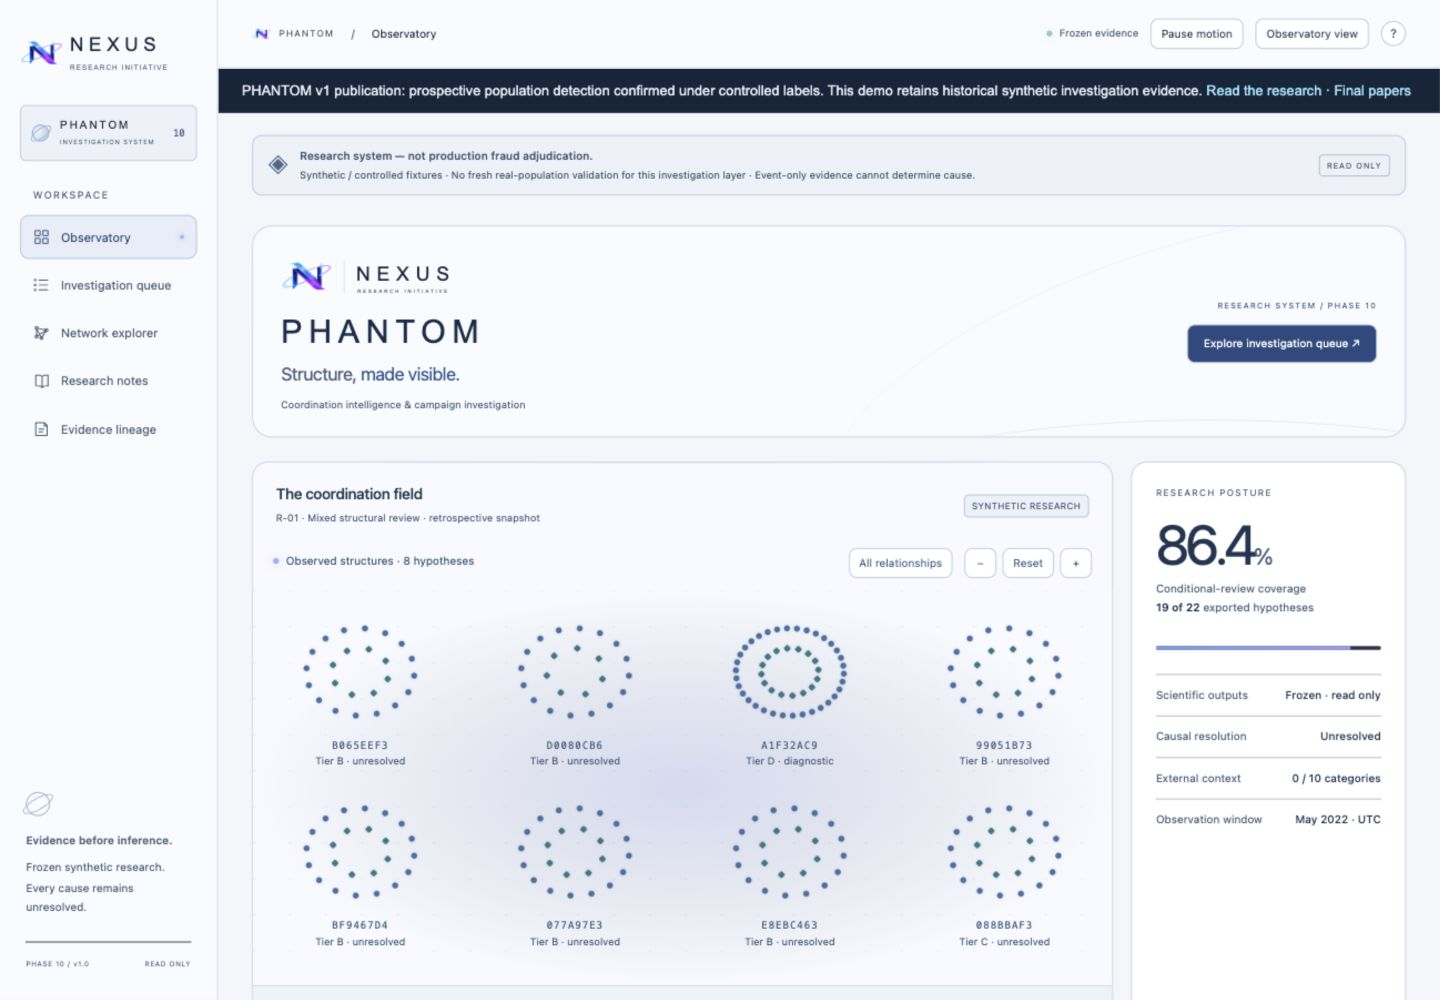
\includegraphics[width=\linewidth]{figures/09_dashboard.png}\caption{Upper Observatory view in the public presentation, captured from unchanged historical synthetic evidence. NEXUS branding and publication navigation are presentation changes only. The 19/22 coverage card concerns exported hypotheses, not real-world accuracy or resolved causes.}\end{figure}

Receipts record 190 fidelity checks, 113 equivalence/filtering checks, 3,392 browser checks, 234 branding/academic/export checks and 14 representative contrast checks: 3,943 in total. They include 132 detail-view combinations, 22 academic exports and 48 academic route/width combinations. These support tested software fidelity and function. They are not independent scientific observations, complete accessibility certification, analyst evaluation or production reliability evidence. \claims{C33--C37}

\section{Prospective Sealed Final Evaluation}
\label{sec:final}
\subsection{Commitment, amendment and execution boundary}
The scientific system and Phase 11 PRE-FINAL manuscripts were frozen before the final population was materialized or scored. The original commitment fixed the source, September 1 inclusive--September 29 exclusive 2026 UTC window, eligibility, exclusions, sampling seed 41290, construction seeds 41291--41293, detector, null, threshold, metrics and acceptance gates. This is a locally recorded prospective commitment, not a claim of registration in an external registry or independent timestamp custody.

Preflight found that the literal \texttt{final412} randomization namespace lacked an executable mapping in the inherited constructor. The original attempt was declared invalid before scoring and remains permanently preserved. Phase 12A defined one deterministic mapping for enrollment, catalog ordering and timestamps, checked it on invented inputs, and resealed it before any final histories were accessed. The amendment did not select among mappings using final outcomes. It preserved the existing scientific parameters and made the namespace semantics explicit; it must not be described as proof that the original commitment was already executable.

A second pre-access issue concerned execution packaging. The first execution lock preceded completion of acquisition, selection, truth-separation and evaluation adapters. Acquisition paused during archive-header indexing; no final event columns, selected population, assignments or scores existed. A superseding lock bound the completed execution files after toy and non-final equivalence checks. Header requests therefore preceded the governing lock, whereas final event access followed it. Both locks survive. The supplement gives the sequence and digest identifiers without exposing protected source records.

\subsection{Population and frozen procedure}
The committed ListenBrainz snapshot supplied 4,032 selected listeners in 42 groups of 96, with 3,714,102 original observed events during September 1--28, 2026 UTC. Three construction seeds and three difficulty levels per group yielded $42\times3\times3=378$ matched pairs and 756 worlds. This is distinct from the May 2022 external-validation population and its 4,004,802 original events. Pair members share histories; repeated worlds share groups and intervention mechanics. The final labels remain synthetic intervention labels, and real listeners are not labelled fraudulent. \claims{F01--F03}

The population-level detector retained its exact schedule selector, 4,095 local-null draws, null seed 41101 and robust-excess threshold of 3.0. No final population was used to fit or revise PHANTOM. Predictions were frozen before the evaluator joined them to protected condition labels. The canonical scientific evaluation ran once; its deterministic verification replay is a reproducibility check, not a second independently sampled experiment.

\subsection{Confirmed results and conditional uncertainty}
Mean block AUC and pooled AUC are both 1.000. All 378 treatment worlds alert and no matched control world alerts. Every group has nine treatment and nine control worlds; worst-block control burden is 0.0\%. All 18 applicable scientific gates pass, and all 756 independent replay worlds are confirmed. External-population transfer therefore extends prospectively to this committed controlled population, while the graph and investigation layers retain their separate historical evidence. \claims{F04--F08}

\begin{table}[!htbp]\centering\small
\caption{Prospective final results, confirmed from immutable frozen outputs. Intervals and the upper bound are conditional outputs of the committed procedure.}
\begin{tabularx}{\linewidth}{@{}Xr@{}}\toprule
Measure & Confirmed result\\\midrule
Mean block / pooled AUC & 1.000 / 1.000\\
Treatment alerts / treatment worlds & 378 / 378\\
Control alerts / control worlds & 0 / 378\\
Worst-block control burden & 0.0\%\\
Equal-block upper 95\% control bound & 0.0\%\\
Conditional AUC interval & [1.000, 1.000]\\
Conditional treatment-detection interval & [1.000, 1.000]\\
Conditional control-mean interval & [0.000, 0.000]\\
Applicable scientific gates & 18 / 18 PASS\\
Independent replay worlds confirmed & 756 / 756\\\bottomrule
\end{tabularx}\end{table}

\fig{10_prospective_final.pdf}{Prospective September result. Real observed listening histories; controlled intervention labels. Each point denotes one of 42 groups with nine worlds per arm. All plotted values are frozen aggregates; no new detector execution or null draws were used.}{1}{fig:final}

The predeclared whole-block uncertainty procedure produces AUC and treatment-detection intervals of $[1.000,1.000]$, control-mean interval $[0.000,0.000]$, and equal-block upper 95\% control bound 0.0\%. These describe the observed controlled population and resampling procedure. Dependence within pairs and groups, shared source context and an unchanged planting family remain. A bootstrap of uniformly perfect observed groups cannot reveal unobserved failure mechanisms. Zero observed control alerts does not establish zero natural-population alert probability. \claims{F09}

\subsection{Receipt failure and post-final forensic confirmation}
The originally locked verifier completed independent replay and reached receipt writing, then failed because a NumPy boolean was not serializable by its JSON writer. It did not complete normally. The partial receipt, traceback and invalid-result disposition remain unchanged; unsaved in-memory checks are not retrospectively assumed to have passed. This was a non-scientific receipt failure after scientific execution, not a failed scientific comparison. \claims{F10}

A separate post-final forensic verifier operated solely on immutable original and replay artifacts. It confirmed all 756 worlds, reproduced every provisional final metric exactly and confirmed all 18 scientific gates. It did not rerun population selection, treatment/control construction, the detector or null generation; change thresholds, seeds or scientific code; or modify predictions. Two forensic tooling incidents, involving library initialization and an incorrect artifact-layout expectation, were also retained. Their correction did not change the scientific equality rules. ``Independent'' here means a separate implementation/fresh process, not a different institution or human evaluator. \claims{F11--F12}

\subsection{Interpretation}
The final establishes prospective controlled separation by the frozen population detector on the committed source population. It does not establish real-world fraud classification, manipulative intent, causal attribution, bot identification, unrestricted stream coverage, production alert rates, analyst effectiveness, enforcement suitability or production readiness. The shared-stimulus and causal-twin failures remain relevant because a new successful test of the same planting family does not supply missing causal information. The final population is now consumed evidence and may never be described as unseen for a new method.

\section{Failures as design constraints}
\begin{table}[tbp]\centering\small
\caption{Failure/remediation summary. A later scope change does not retroactively pass an earlier failed gate.}
\begin{tabularx}{\linewidth}{@{}p{.17\linewidth}YYY@{}}\toprule
Problem & Failure & Implication & Change\\\midrule
Synthetic origin & Generated neutrals separated & Detector could identify simulator & Origin and neutral gates\\
Sessions & All source groups had ten rows & Unvalidated behavioral meaning & Session-free designs\\
Catalog shortcuts & Catalog exposed source origin & Graph gains were confounded & Matched actor marginals\\
Duplicates & 20/180 pairs changed keys & Preprocessing changed support & Collision-safe construction\\
Raw calibration & 22/180 controls alerted & AUC did not rescue threshold & Local median/MAD scaling\\
Graph null & High control burden & Reconstruction could be spurious & Presence, conditioning, pooling\\
Hybrid & Actionable F1 fell to 0.5357 & Veto removed useful evidence & Retain core\\
Common stimulus & Every shock control alerted & Structure did not identify intent & Alternatives and provenance\\
Shifted overlap & F1 0.3636 & Parent association failed & Explicit support boundary\\
Scalar priority & IDs and ambiguity changed rank & Ordering implied preference & Equal-priority sets\\\bottomrule
\end{tabularx}\end{table}
Some failures have representation fixes; others demand a different statistical question. Duplicate presence is a representation issue. Null conditioning refines what departures count as unusual. Causal twins expose missing information that a transformation of the same events cannot restore. A responsible research system must distinguish these categories rather than turning every unresolved requirement into a stronger score.

The chronology supplement records objectives, hypotheses, methods, gates, decisions and resulting changes for every stage. It retains rejected approaches and the conditions under which later work proceeded. The main narrative is organized by scientific problem so that readers can assess the accepted method without navigating internal phase numbers.

\section{Reproducibility and permissible release scope}
The source map indexes authorized reports, frozen metrics, code and design artifacts. The claim ledger records exact wording, line or JSON field, denominator, population, acceptance status, limitations and permitted placement. The citation ledger records primary-source checks and exact supporting claims. Figures transcribe frozen aggregates or provide labelled conceptual diagrams; they do not generate new scientific observations.

\begin{samepage}
Relevant implementations include \path{phase4_11/src/local_null.py} and \path{phase5_1/src/pooling.py}, the latter depending on its frozen detector module. The accepted pooling SHA-256 begins \texttt{50226721} and ends \texttt{764979}; the source map retains the full digest. Hashes establish identity, not validity. Reproduction also needs runtime versions, seeds, canonicalization and permitted data access. Rebuilding this paper is not rerunning the science.
\par\end{samepage}

Phase 13 performs record, hash and arithmetic checks on frozen results. It does not run or tune scientific producers. Full historical reproduction requires authorized source access. The public package supplies aggregate figure rebuilding and synthetic teaching examples; these do not reproduce the full experiment. Protected raw histories, evaluator truth and private logs are excluded.

The repository specification is an allowlist: manuscripts, references, figures, cleared selected code, entirely synthetic toy data and a sanitized frozen dashboard demonstration after release review. It excludes raw datasets, protected truth, final material, private identifiers, credentials and orchestration logs. The toy example illustrates conditional permutation but does not reproduce the reported experiment. Raw datasets and frozen research-code redistribution remain restricted; the release matrix defines the allowed documentation and synthetic-demo subset. No open-source license is granted by publication preparation.

\section{Limitations and next scientific work}
\paragraph{Labels and causality (construct validity).} Treatment labels identify planted assignment changes, not dishonest listeners. The event schema omits exposure, referral and organizer provenance. Causal twins demonstrate one exact ambiguity; they do not characterize the prevalence of indistinguishable real cases. Structural significance cannot be reinterpreted as a calibrated probability of intent.

\paragraph{Mechanism and support (external validity).} The exact recurring-schedule selector is aligned with the controlled intervention. Passing invariance checks establishes that the identified shortcuts were addressed, not that the benchmark is generally difficult. Coverage of ordinary streams, unseen coordination mechanisms and natural-process exchangeability remain unknown. The final changes source population and period under the same intervention family.

\paragraph{Dependence and reconstruction (internal and external validity).} The final has 42 source groups, not 756 independent populations. Whole-group resampling retains the observed dependence unit but cannot establish independence across groups or uncertainty over unseen mechanisms. The graph holdout comprises two historical blocks; later stress tests reuse development histories. Prospective detector results do not externally validate reconstruction or investigation coverage.

\paragraph{Comparisons and utility (comparative and operational validity).} No matched published-method baseline establishes superiority. No analyst study, production deployment, enforcement outcome or unrestricted throughput measurement is available. Incomplete parent coverage remains a limitation even when a candidate is reviewable. The dashboard implements an evidence contract; it does not validate its benefit.

\paragraph{Rights and reproducibility (auditability).} Public reproduction covers equations, aggregate figures and wholly synthetic teaching examples. Full experiments require authorized source access; raw histories, protected final truth and uncleared research code are excluded. Local commitments and process-separated verification provide an audit trail, not independent institutional attestation. Detailed seeds, selectors, gates and the complete verification incident are retained in the supplement. Any new comparator experiment or method change requires a separately committed study; the final population is already consumed.

\section{Conclusion}
PHANTOM v1 demonstrates conditional detection of planted coordination across observed listening populations and bounded reconstruction of member and target structure. The prospective final evaluation confirmed perfect separation within its committed controlled procedure; the preserved verifier incident changes the verification history, not the reproduced scientific values. That result does not erase origin confounding, threshold failures, rejected hybrid designs, common-stimulus failures or overlap ambiguity. These findings explain the final task: provide inspectable evidence and investigation priorities while withholding unsupported causal judgments. Matched comparative evaluation, broader support coverage, independent contextual evidence and analyst studies remain future research. Any method change belongs to PHANTOM v2; the consumed September population cannot serve as unseen evidence for it.

\section*{Authorship and AI assistance}
Nischit Girish Kumar is the sole human author. NEXUS Research Initiative denotes independent research, not institutional sponsorship. \textbf{AI Assistance Disclosure:} AI-assisted tools supported selected engineering tasks, with minor assistance in documentation and manuscript preparation. Nischit Girish Kumar directed the research, system architecture, experimental design, validation, and final technical decisions and assumes responsibility for the work.
\begingroup\small\setlength{\bibsep}{5pt}\bibliographystyle{plainnat}\bibliography{references}\endgroup
\end{document}
